\subsection{Heat Transfer}
\subsubsection{Combustor [Cameron Ellis]}

The combustor consisted of a rotating detonation engine surrounded by an inner and outer wall that were each coated in TBC and regeneratively cooled. Heat transfer through the walls was calculated using a modified form of Bartz equation in order to calculate the heat transfer coefficient hg inside the combustor. Equation \ref{eqn:modBartz} shows the standard form of Bartz equation for a rocket nozzle.

\begin{equation}
h_g = \left[ \frac{0.026}{D_t^{0.2}}\left(\frac{\mu^{0.2}C_p}{Pr^{0.6}}\right)_{ns} \left( \frac{(p_c)_{ns}g}{c^*} \right)^{0.8} \left(\frac{D_t}{R}\right)^{0.1} \right] \left(\frac{A_t}{A}\right)^{0.9}\sigma
\label{eqn:modBartz}
\end{equation}

Where the $ns$ subscript denotes values of the gas inside of the combustor, and where sigma is the correction factor denoted by Equation \ref{eqn:longSigma}.

\begin{equation}
\sigma=\frac{1}{\left[ \frac{1}{2} \frac{T_{wg}}{(T_c)_{ns}} \left( 1 + \frac{\gamma - 1}{2}M^2\right)+\frac{1}{2}\right]^{0.68} \left[1+\frac{\gamma-1}{2}M^2\right]^{0.12}}
\label{eqn:longSigma}
\end{equation}

For this combustor, there is no nozzle radius of curvature, denoted by R in the Bartz equation, so the term $\left(\frac{D_t}{R}\right)^{0.1}$ becomes 1. Furthermore, the area of the throat and the area of the combustor are equal since they have the same radius, so the area ratio term $\left(\frac{A_t}{A}\right)^{0.9}$ also becomes 1. Once an $hg$ value was obtained, a guess at the hot side wall temperature, $T_{wg}$ was taken and used to calculate heat flux from the combustor to the surface of the wall. This heat flux was then compared to the heat flux from the liquid coolant to the cold side of the wall, and compared together. The hot side wall temperature then changed iteratively until the two heat flux values matched. This was done across the entire length of the combustor, and was used to find the temperatures of the TBC inside the combustor, the temperature of the metal inside combustor wall, and the temperature of the ethylene in order to make sure boiling would not occur.

\begin{figure}[H]
\begin{center}
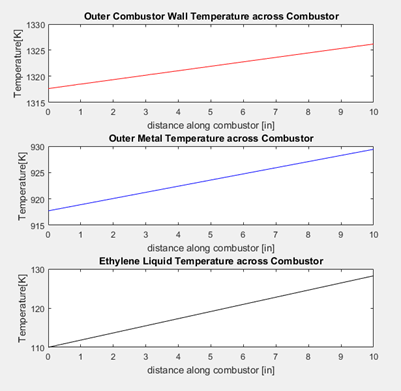
\includegraphics[width=0.6\textwidth]{combustorWallTemps}
\caption{Temperature Range Across Combustor Structure}
\label{fig:combustorWallTemps}
\end{center}
\end{figure}

Figure \ref{fig:combustorWallTemps} shows the temperature of the TBC, inside metal wall, and the ethylene across the length of the combustor. The TBC experiences temperatures of upwards of 1327 K at the hottest points after regenerative cooling is applied. The metal wall experiences up to 930 K, and therefore a material that could withstand those temperatures without going past its deformation temperature had to be selected. Incoloy 800 HT was chosen due to its high heat resistance. At the calculated temperatures, the alloy would be able to work at about 60\% of its intended strength. The TBC coating selected was NAS3-23944, a super TBC created by NASA.

Figure \ref{fig:incoloyPlot} displays the elongation, tensile strength, and yield strength for INCOLOY 800HT for various temperatures. Though at the temperatures the RDE combustor would be operating at would affect the strength of the INCOLOY, it is still within a reasonable operating range for the metal work as intended.


To regeneratively cool both sides of the combustor, the mass flow rate of the liquid ethylene had to be split up between the inner and outer walls. Since the inner wall has a lower surface area, it would need less cooling channels, while the larger outer wall would need more. The cooling channels were split into 100 channels on the inner wall and 120 channels on the outer wall. Each cooling channel has a dimension of 0.215”x0.125” The mass split of the fuel ended up being 48.5\% of fuel going to the inner regenerative cooling, and 51.5\% of fuel going towards the outer regenerative cooling.  This allows the two walls to experience approximately the same heat transfer, so the same thickness of thermal barrier coating would be able to be used on both sides. This was done to ensure that one side would not need to thick a layer of thermal barrier coating and increase the chance of cracking and flaking to take place during combustion.

\begin{wrapfigure}{r}{0.65\textwidth}
\begin{center}
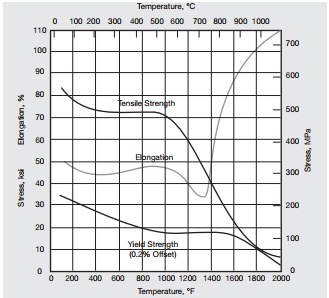
\includegraphics[width=0.6\textwidth]{incoloyPlot}
\caption{Temperature Range Across Combustor Structure \cite{inco}}
\label{fig:incoloyPlot}
\end{center}
\end{wrapfigure}

\subsubsection{Nozzle [Gabriel Diez]}

The data used to design the ablative cooling system on the nozzle was taken from Tick et al \cite{tick}. In the study N2O4 and hydrazine were burned at 830 kPa and exhausted out of a nozzle coated with a 12.5 mm thick layer of silica phenolic ablative. Several parameters were varied in the experiment but in each test the fluid temperature exiting the combustor was 3144 K which lead to surface temperatures on the nozzle of 2644 K. Under these conditions, the time to char through the ablative as well as the erosion rate were measured. The time to char through was above 200s and the erosion rate never exceeded 0.05 mm/s. Since the total burning time of the RDE scramjet is 120 s and the gas temperatures never exceed 2500 K, it can be estimated that no more than 6 mm of ablative will be burned off. Therefore a design with a 12.5 mm thick layer of silica phenolic ablative coating similar to the one used in the Tick et al (1965) study was chosen since it had been proven experimentally to function under harsher conditions for a longer period of time. The ablative coating covers a metal interior support made of titanium for even further protection against any conductive heat transfer. A cross section of the ablative layer is displayed in Figure ( ).

\subsubsection{Wings and Leading Edges [Alberto Marin Cebrian]}
All the temperatures have been calculated for the steady state and for the most demanding operating conditions (cruise, Mach 6.5). The materials used in these exterior surfaces must tolerate high temperatures and a high emissivity is desirable. A higher emissivity will allow the material to reduce the maximum temperature it will have to withstand because it will be able to radiate more heat to the surroundings.

\paragraph{Inlet Cone Tip and Wing Leading Edges}
Infinitely thin surfaces and points are not possible to manufacture. Due to this fact a small normal shock will appear in front of these blunt bodies. This detached normal shock will create a huge deceleration of the flow and the properties of the flow will change significantly, it has been assumed that the air properties ($\gamma$ in particular) will also change as the flow crosses the shock.

Properties after the shock allow us to calculate the Prandtl number at that location

\begin{equation}
Pr=\frac{(\mu_e Cp_e)}{K_e} =0.4574
\end{equation}

Assuming that the boundary layer remains laminar, a similarity solution exists.
\begin{equation}
\frac{du_e}{dx}=\frac{1}{r_n}\sqrt{\frac{2(p_e-p_0)}{\rho_e}}
\end{equation}

The recovery temperature depends on the Prandtl number. For laminar flows the recovery factor is r=sqrt(Pr)
\begin{equation}
T_r=T_e (1+(\gamma_e-1)/2 \sqrt{Pr} M_e^2 )=2082 K
\end{equation}

Convective heat flux on the inlet cone tip
The shape of the blunt cone is approximated to a semi-sphere. The heat flux is given by:

\begin{equation}
\dot{q}=0.763Pr^{0.6}(\rho_e\mu_e)^{1/2}\sqrt{\frac{du_e}{dx}}Cp_e(T_r-T_w)
\label{eqn:tipHeatFlux}
\end{equation}

Convective heat flux on the wing leading edge
The leading edge of the wing has a cylindrical shape with a nose radius equal to half of the thickness of the wing. The heat flux is also given by given by Equation \ref{eqn:tipHeatFlux}.

Radiation heat flux
The radiation heat flux has been calculated with the Stefan-Boltzman equation.

\begin{equation}
\dot{q}_{rad}=\sigma_s (\eta_w T_w^4-T_0^4)
\end{equation}

Steady state solution is reached when $\dot{q}=\dot{q}_{rad}$.


*This value has been guessed and based on the manufacturing tolerance it may change significantly. On the one hand, a bigger nose radius will decrease the temperature of the cone tip but it will decrease the performance of the inlet adding more drag. On the other hand, a smaller nose radius will be beneficial for the inlet performance but it will increase the temperature of the inlet cone. This value must be small enough not to affect significantly the inlet performance but big enough to be manufactured and get a temperature that lies inside the operating range of the material.

\paragraph{Wing Surface Temperature}
In order to obtain the temperature field over the wing of the aircraft the following assumptions have been made.
	The angle of attack of the vehicle is very small during the flight. This fact allows us to simplify the physics of the problem assuming that the angle of attack ($\alpha$) is zero. In reality the angle will be different from zero and a compression oblique shock wave will appear for the lower part of the wing and an expansion wave will be developed in the upper surface. These waves will be very weak and will not change significantly the results of this analysis as soon as the angle of attack keeps being small enough.
	The wings are long and slender. Flat plate approximation has been used to calculate the heat fluxes at different sections of the wing.
	1-D flow. The velocity of the flow can be simplified to $\overrightarrow{v}=(u,0,0)$.
	
Some important non-dimensional parameters that control the physics of this problem are the Reynolds number, the Prandtl number and the Nusselt number.
The Reynolds number relates the inertial and viscous effects. It determines the change from laminar to turbulent flow in the boundary layer. For a flat plate, the transition Reynolds number from laminar to turbulent is 500,000.
\begin{equation}
Re_x=\frac{\rho u x}{\mu}	
If   Re_x<500,000, Laminar boundary layer
	If   Re_x>500,000, Turbulent boundary layer
\end{equation}

The Prandtl is a dimensionless parameter representing the ratio of diffusion of momentum to diffusion of heat in a fluid. [2]

\begin{equation}
Pr=\frac{\mu Cp}{K}
\end{equation}

The recovery factor (r) depends on both, Prandtl number and Reynolds number.

\begin{equation}
\begin{split}
r=\sqrt{Pr} \text{  For laminar B.L.}	\\
r=Pr^{1/3} \text{  For turbulent B.L.}
\end{split}
\end{equation}

The Nusselt number is the ratio of convective hat transfer with respect to conduction. The Nusselt number depends on the other two dimensionless parameters (Prandtl number and Reynolds number).

\begin{equation}
Nu_x=\frac{h_g x}{K}
\end{equation}

\begin{equation}
\begin{split}
Nu_x=0.332\sqrt{Re_x} Pr^{1/3}	\text{  For laminar flows} \\
Nu_x=0.0296Re_x^{0.8} Pr^{1/3}	\text{  For turbulent flows}
\end{split}
\end{equation}

With the Nusselt number and the axial position it is possible to obtain the convective heat transfer coefficient $h_g$.

\begin{equation}
h_g=\frac{K Nu_x}{x}
\end{equation}

Note that this analysis is not valid for x=0 where the leading edge is located ($h_g$ is infinite there).
The convective heat flux is 

\begin{equation}
\dot{q}=h_g (T_r-T_w)
\end{equation}


Steady state is reached when the heat dissipated by radiation equals the heat inflow due to convection $\dot{q}=\dot{q}_{rad}$
In order to get the temperature contour of the wing, the wall temperature of the wing has been calculated in numerous locations along the wing.
